\documentclass[11pt]{article}
\usepackage{amsmath, amssymb}
\usepackage{geometry}
\geometry{margin=1in}
\usepackage{fancyhdr}
\usepackage{lastpage}
\usepackage{parskip} % Better paragraph spacing
\usepackage{titlesec} % Better section formatting
\usepackage{graphicx}
\usepackage{float}
\usepackage[most]{tcolorbox}
\usepackage{lmodern}
\usepackage{caption}
\usepackage{hyperref}
\usepackage{listings}
\usepackage{xcolor}

\definecolor{codegreen}{rgb}{0,0.6,0}
\definecolor{codegray}{rgb}{0.5,0.5,0.5}
\definecolor{codepurple}{rgb}{0.58,0,0.82}
\definecolor{backcolour}{rgb}{0.95,0.95,0.92}

% Define code styling
\lstdefinestyle{mystyle}{
    backgroundcolor=\color{backcolour},
    commentstyle=\color{codegreen},
    keywordstyle=\color{magenta},
    numberstyle=\tiny\color{codegray},
    stringstyle=\color{codepurple},
    basicstyle=\ttfamily\footnotesize,
    breakatwhitespace=false,
    breaklines=true,
    captionpos=b,
    keepspaces=true,
    numbers=left,
    numbersep=5pt,
    showspaces=false,
    showstringspaces=false,
    showtabs=false,
    tabsize=2
}

\lstset{style=mystyle}

% Define commands for reusable content
\newcommand{\coursename}{COM-402 Information Security and Privacy}
\newcommand{\lecturedate}{\today}
\newcommand{\professor}{Mathias Payer}

\hypersetup{colorlinks=true,linkcolor=blue,urlcolor=blue}

% Configure section spacing
\titlespacing*{\section}{0pt}{2ex plus 1ex minus .2ex}{1.5ex plus .2ex}
\titlespacing*{\subsection}{0pt}{1.5ex plus 1ex minus .2ex}{1ex plus .2ex}
% Header / Footer
\pagestyle{fancy}
\fancyhf{}
\fancyhead[L]{\coursename}
\fancyhead[R]{Lecture \lecturenum}
\fancyfoot[L]{EPFL - Computer Science}
\fancyfoot[C]{Author: Jonathan Dutoit}
\fancyfoot[R]{Page \thepage\ of \pageref{LastPage}}

\begin{document}

\begin{center}
  {\large EPFL - Computer Science} \\[0.5em]
  {\Large \textbf{\coursename}} \\[0.5em]
  {\large Lecture \lecturenum\ --- \lecturedate} \\[0.5em]
  {\large Author: Jonathan Dutoit} \\[0.5em]
  {\large Professor: \professor} \\[0.5em]
\end{center}

\vspace{2cm}

\begin{center}
  {\LARGE \textbf{Trusted Computing}}
\end{center}

\vspace{1cm}

\section*{Learning Goals}

\begin{itemize}
	\item Understand \textit{\textbf{the need}} for trusted computing
	\item Learn the \textbf{\textit{guarantees}} provided by \textit{\textbf{trusted computing}}
	\item Understand the threat model
	\item Know some \textbf{\textit{key technologies}} used in trusted computing
	\item Understand how violating the threat model can break trusted computing
	\item Understand the basics of \textit{\textbf{side-channel attacks}}
\end{itemize}

\section*{Can you trust applications?}

All modern systems built on abstractions

Software systems like
\begin{itemize}
	\item Operating systems / Hypervisors
	\item Compilers
	\item Runtime/static libraries
\end{itemize}

Are extremely complex and maintained by untrusted parties (even open source has bugs)

\section*{What about Hardware?}

Computer is owned or controlled by another party, e.g., in Cloud computing

Hardware is extremely complex and was built by an untrusted party (e.g., Intel, ARM, Apple) and manufacture by a fab (e.g., TSMC)

Other, untrusted applications run on the computer, e.g., cloud computing, smartphone

\textbf{Better question: why trust a computer?}

\section*{Can we trust the hardware?}
\begin{tcolorbox}[
  colback=gray!15,     % background color
  colframe=black!50,    % border color
  boxrule=1pt,       % border thickness
  arc=3mm,             % rounded corners
  left=4mm, right=4mm, top=2mm, bottom=2mm % padding
]
\textbf{Trusted Hardware}

\vspace{0.3cm}

"A piece of hardware can be trusted, if it always behaves in the expected manner for the indented purpose" - Trusted Computing Group \\

\textbf{Trusted Computing}: Trusted software (component, verified, analysed) running in a secure hardware container. The guarantees we get is that no one can extract secrets.
\end{tcolorbox}

\section*{Trusted Hardware Key Properties}

\begin{itemize}
	\item \textbf{Attestation}: hardware proves that it does what it's supposed to do
	\item \textbf{Isolation}: privileged code cannot observe computation
	\item \textbf{Sealing}: hardware encrypts data so it can only be accessed when the system meets specific trusted conditions
\end{itemize}

\subsection*{Attestation}

\textbf{Proves that system is in a specific state to an authorized party.}

Attest to a remote authorized party. Is this computer running the correct code?

% Quick centered image
\begin{figure}[H]
    \centering
    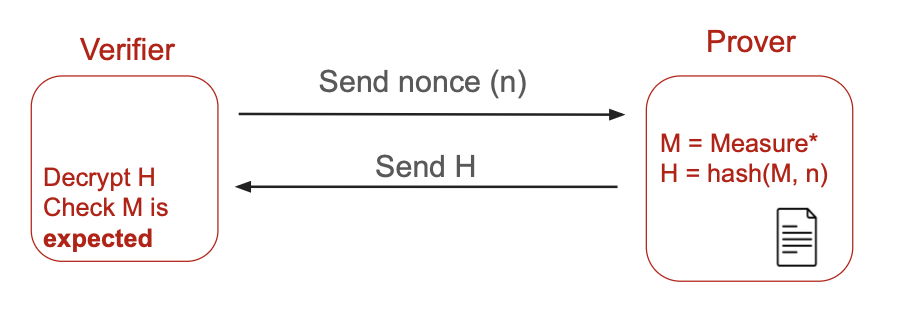
\includegraphics[width=0.8\textwidth]{attestation}
    \label{fig:LABEL}
\end{figure}

\textit{For now measure is magic, ensures safety}

\subsection*{Isolation}

\textbf{Constraints who and what can be accessed (access control)}

\begin{minipage}{0.6\textwidth}
\begin{itemize}
	\item Unauthorized applications cannot access/write region
	\item Trusted hardware offers \textbf{one well-identified entry-points} to interact with software (to ensure CFI)
\end{itemize}

The \textbf{well-identified} is important to avoid attackers to access any arbitrary access to the application's code (Control Flow Integrity). Imagine a \verb|memcpy| function that could be accessible, hence attackers could use that to copy all fingerprints...

\end{minipage}
\hfill
\begin{minipage}{0.4\textwidth}
\centering
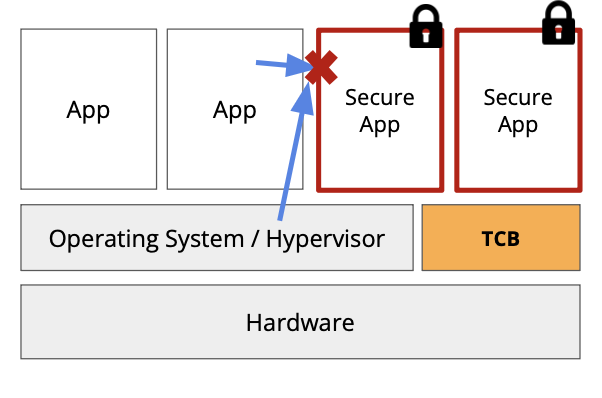
\includegraphics[width=\linewidth]{isolation}
\end{minipage}

\subsection*{Sealing}

\textbf{Protects private information by binding it to platform configuration or the state.}

\textit{Store information outside of the trusted environment}

\begin{minipage}{0.4\textwidth}
\textbf{\textcolor{red}{X}} might be the state of the module, or configuration information including the used software and hardware.  \\

Enables secure persistent storage in untrusted memory.
\end{minipage}
\hfill
\begin{minipage}{0.6\textwidth}
\centering
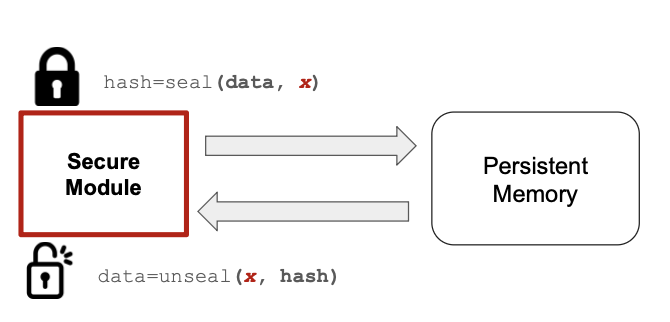
\includegraphics[width=\linewidth]{sealing}
\end{minipage}

Sealing encrypts data with keys stored inside the TPM, and this data can only be "unsealed" when the TPM verifies that the current system configuration matches the predefined conditions. This helps protect against unauthorized access or tampering, ensuring the integrity and confidentiality of sensitive data.

\section*{Trusted Hardware}

Any hardware that has been certified to perform \textbf{\textit{according to a certain set of requirements}} under \textbf{\textit{strong adversarial conditions}}

\begin{itemize}
	\item TPM chip
	\item Hardware Security Module
	\item Intel SGX
\end{itemize}

\textbf{Hardware answers the "how" trusted computing can be achieved}

\subsection*{Trusted Platform Module (TPM)}
% Quick centered image
\begin{figure}[H]
    \centering
    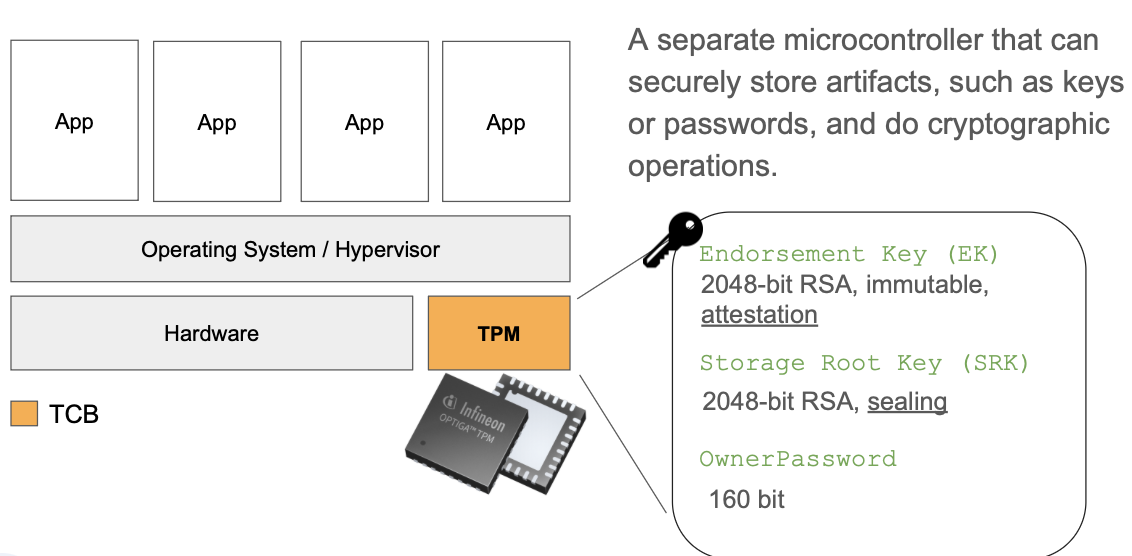
\includegraphics[width=1\textwidth]{tpm}
    \label{fig:LABEL}
\end{figure}

\subsection*{TPM: Attestation}

These chips include Platform Configuration Registers (PCR)

\begin{itemize}
	\item PCRs are initialized at \underline{boot time} to default value (e.g., 0)
	\item They are \underline{append only}
	\item We can store measurements in these PCRs registers.
	\item \verb|TPM_extend(D)|: Adds a measurement to TPM
	\item \verb|TPM_PCRREAD(n)|: returns \verb|PCR[n]|
\end{itemize}

\textbf{Example}: Secure boot is a perfect example.

% Quick centered image
\begin{figure}[H]
    \centering
    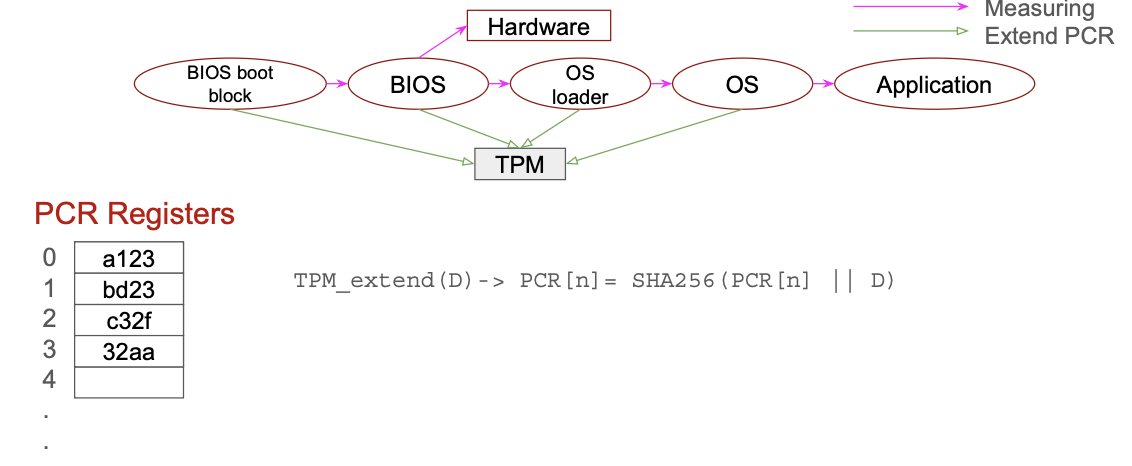
\includegraphics[width=0.8\textwidth]{tpm-attestation}
    \label{fig:LABEL}
\end{figure}
In the \textbf{\textit{BIOS boot block}}: it loads the BIOS in memory, then asks the TPM to a SHA-256 version of the BIOS (which is a few megabytes) and we compare it to the expected value (which could be hardcoded in hardware, an extension could be if the TPM checks if the BIOS has been \textit{\textbf{signed}}). If yes, we start the \textbf{BIOS}. This is to avoid attacks on the BIOS. 

\subsection*{TPM: Sealing}

\textbf{Encrypts a full disk volume}

Store: \verb|TPM_Seal(keyhandle, PCRValues, Data)| 

Recover: \verb|TPM_Unseal()|

tpm.msc:
\begin{itemize}
	\item Auto generates 160-bit \textcolor{green}{OwnerPassword}
	\item Stored on TPM and in file \verb|computer_name.tpm|
\end{itemize}
\textcolor{red}{Volume Master Key} (VMK) encrypts disk volume key

\section*{Hardware Secure Modules (HSMs)}

External cryptography-oriented device to manage secrets
\begin{itemize}
	\item generating keys
	\item encrypting and decrypting data
	\item and creating and verifying digital signatures
\end{itemize}

Tamper-resistant hardware device (opening it to steal data won't work)

To flush all data, just delete the key (it's all encrypted with a single key) which is \verb|O(1)| operation. Other alternatives are magnesium, magnets, ... 

% Quick centered image
\begin{figure}[H]
    \centering
    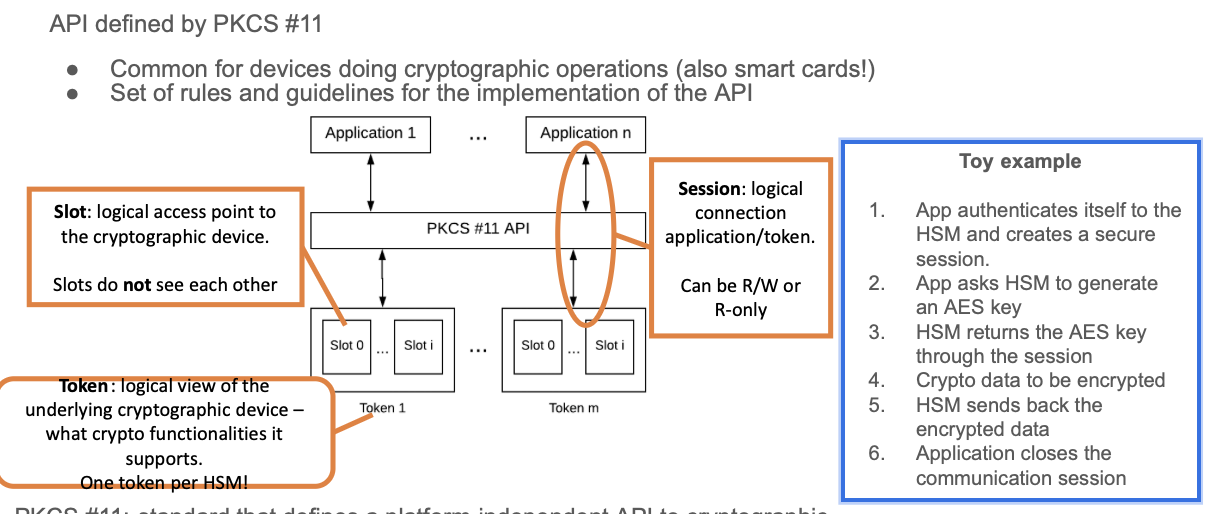
\includegraphics[width=1\textwidth]{hsm}
    \label{fig:LABEL}
\end{figure}

PKCS #11: standard that defines a platform-independent API to cryptographic tokens, such as hardware security modules (HSM) and smart cards.

\section*{Intel SGX}
% Quick centered image
\begin{figure}[H]
    \centering
    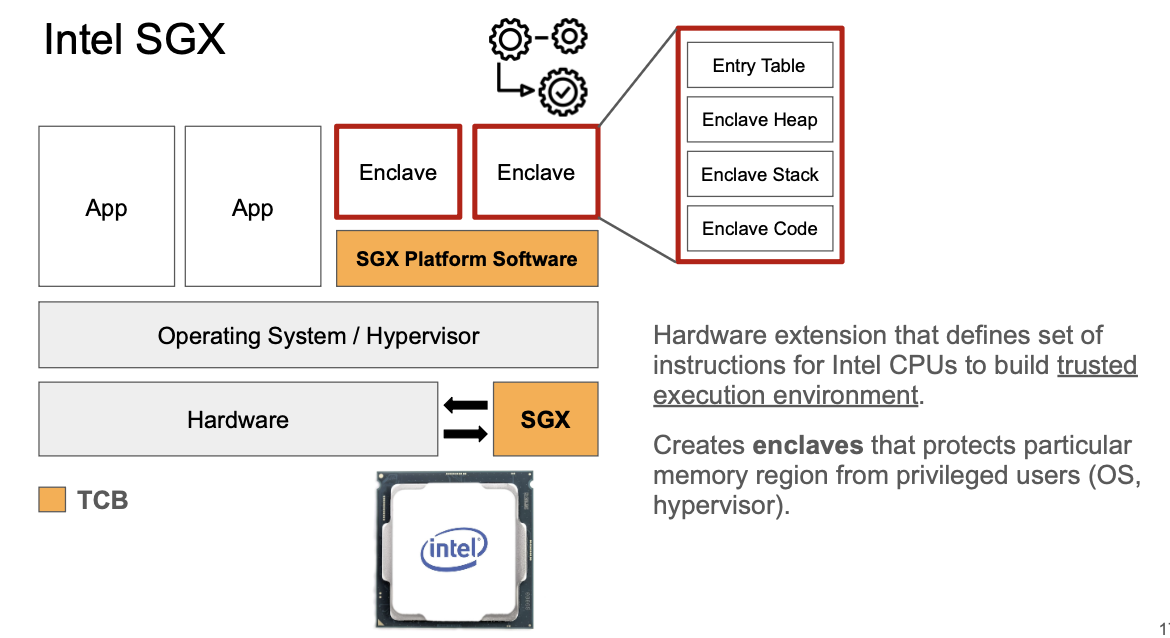
\includegraphics[width=1\textwidth]{intel}
    \label{fig:LABEL}
\end{figure}


The \textcolor{red}{enclave} gives \textbf{isolation}.

The enclave cannot call \verb|syscall| functions, it can copy the data already encrypted outside (into the untrusted application)

SGX provides two types of attestation:
\begin{itemize}
	\item \textbf{Local attestation}: an enclave can check other enclave's integrity
	\item \textbf{Remote attestation}: remote party check an enclave's integrity.
\end{itemize}

\section*{Signal}

Signal is a messaging application designed to offer strong(er) privacy protection

\begin{itemize}
	\item End-to-end encryption
	\item Keys stored on the device
	\item (Mostly) open source
	\item Independent, not for profit (funded by donations)
\end{itemize}

\begin{tcolorbox}[
  colback=gray!15,     % background color
  colframe=black!50,    % border color
  boxrule=1pt,       % border thickness
  arc=3mm,             % rounded corners
  left=4mm, right=4mm, top=2mm, bottom=2mm % padding
]
\textbf{Problem}

\vspace{0.3cm}

How to do private contact discovery? In other words, how do find intersection between "Who in my contacts uses Signal" and "Signal Users" database.
\end{tcolorbox}

Threat model: Who do you want to protect against? Why? \\
1. Protect from Signal
\begin{itemize}
	\item \textbf{Privacy}: Users do not want to leak any information to Signal about who their contacts are (especially those not using Signal)
\end{itemize}

\textcolor{red}{\textbf{Threat Model}: Protect privacy of contacts}
\begin{itemize}
	\item \textbf{Access Control?}: No, we cannot... same problem as before, where is the hardware secure module?  Signal is a threat in the threat model
	\item \textbf{Cryptography?}: We encrypt the set of contacts in the message and decrypts in the signal application. Oh wait, The idea was \textbf{not} to show the contacts signal. 
	\item \textbf{Better Cryptography}? Signal's set is very big. PSI does not scale. (PSI = Private Set Intersection)
	\item \textbf{Intel SGX}: SGX secure enclave creates an isolated memory region. Cryptographic keys from Signal. Computer intersection with PSI. \\
	
\textcolor{orange}{\textbf{Challenge}: how does the phone know the enclave runs the right program?}

\textcolor{green}{The enclave is open source and the user (phone) can compute (and check) the hash used in attestation}
	\item With \textbf{Better} Intel SGX: 
		% Quick centered image
		\begin{figure}[H]
		    \centering
		    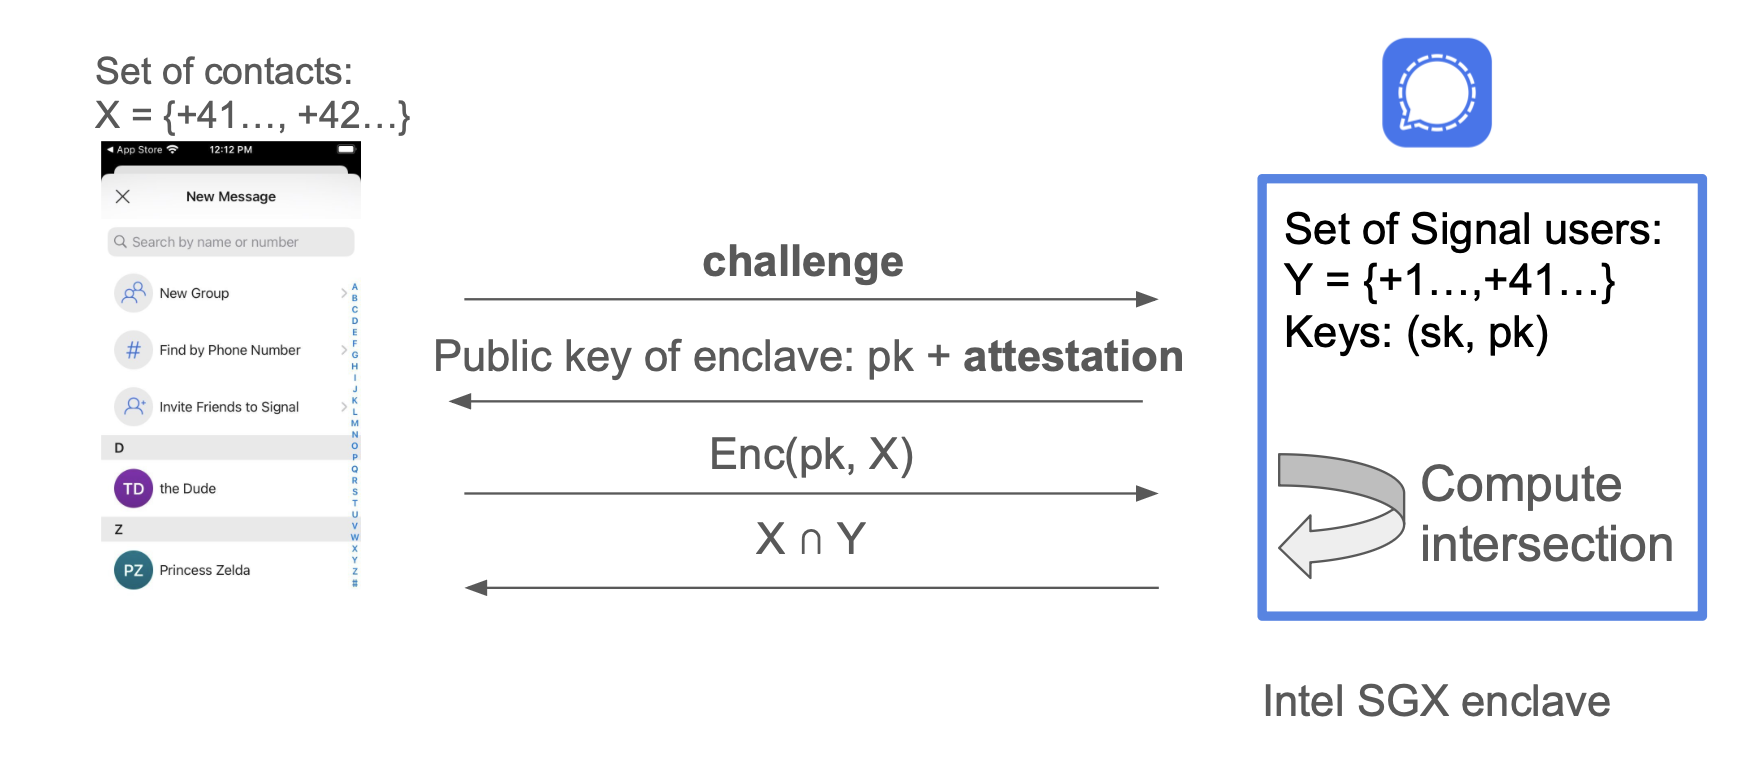
\includegraphics[width=0.8\textwidth]{better-intel-sgx}
		    \label{fig:LABEL}
		\end{figure}
\end{itemize}

\subsection*{Signal: Using Sealing to Store Keys}

% Quick centered image
\begin{figure}[H]
    \centering
    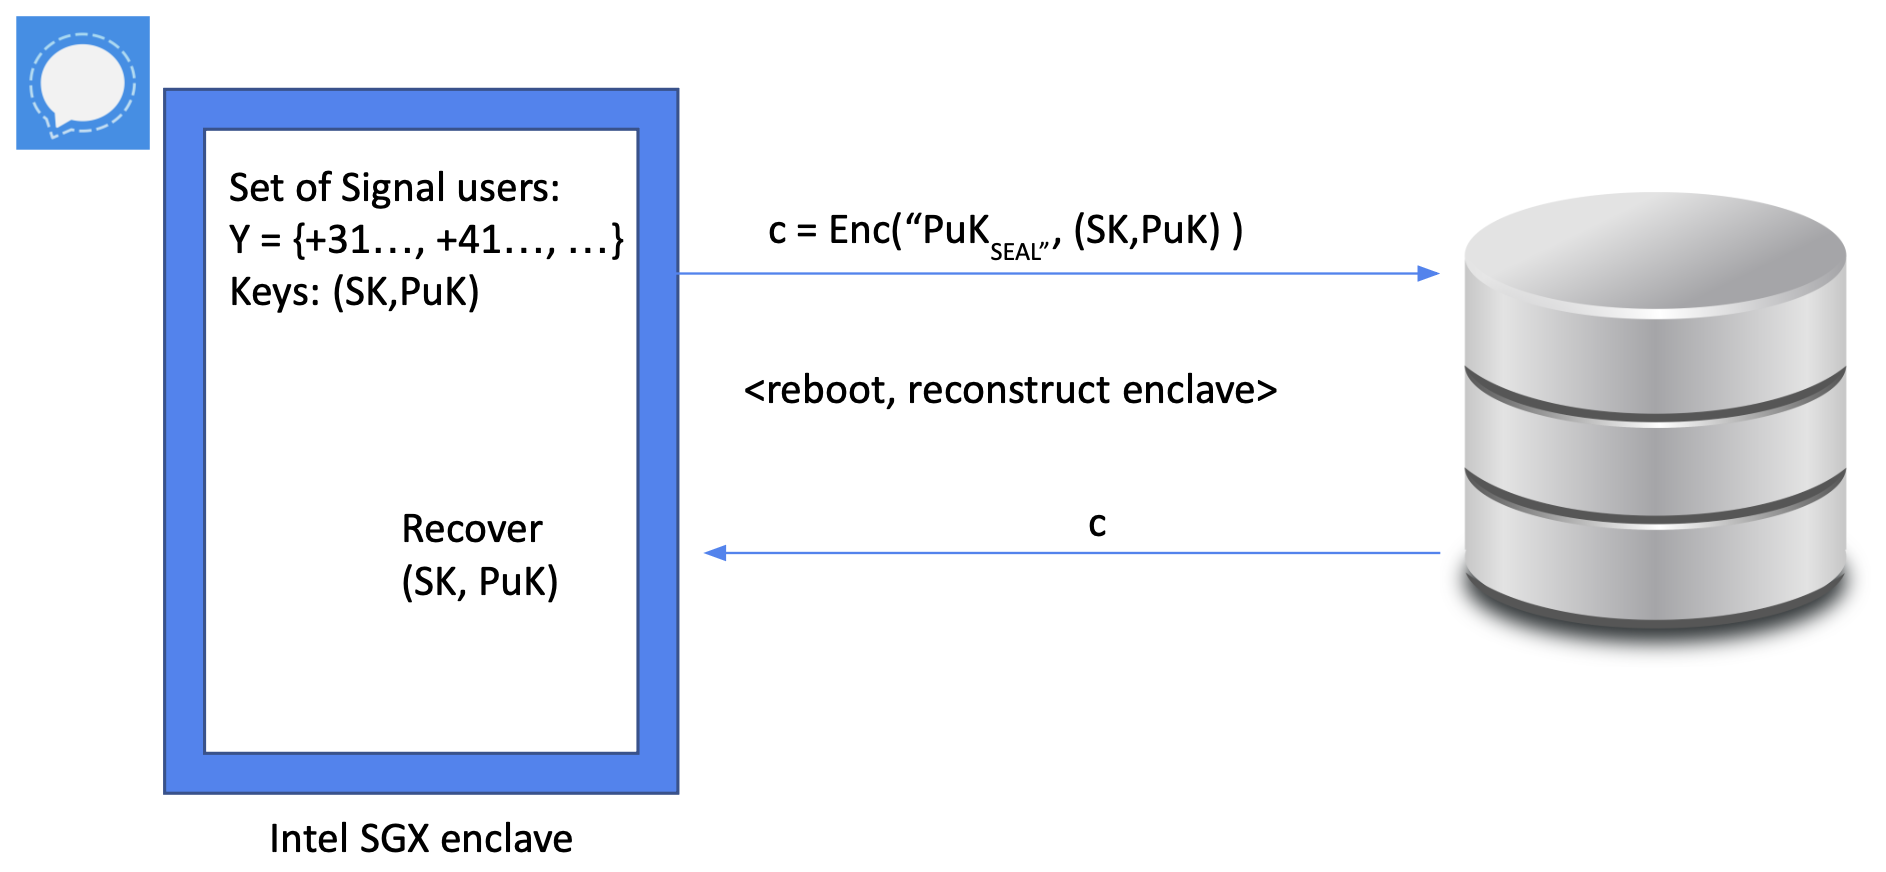
\includegraphics[width=0.8\textwidth]{signal-sealing}
    \label{fig:LABEL}
\end{figure}

\section*{iPhone Backups}

Problem statement: we want users to be able to backup their data to the cloud; the user should be the \textbf{only one} that can recover their data

\textbf{Threat model}

Who do you want to protect against/why?
\begin{itemize}
	\item Other users
	\item Cloud provider
	\item Apple
	\item External parties
\end{itemize}

Adversaries have lots of computational power!

What about government issues?

\subsection*{Problem: Offer cloud backups for data but guarantee that users retain \textit{exclusive} access}

\textcolor{red}{\textbf{Threat Model}: Other users and cloud provider as well as Apple and external parties}

\begin{itemize}
	\item \textbf{Access Control}:
		\begin{itemize}
			\item Problem: \textbf{\textit{Location of the Hardware Security Module (HSM)}}: Apple and the Cloud are in your threat model!
			\item Problem: \textbf{\textit{Access control for data}}: Even if Apple and the Cloud \textit{were trusted} for running the system, access control just prevents other users and third parties from accessing the data. (And this does not apply to third parties with subpoenas.)
\end{itemize}
	\item \textbf{Cryptography}: what if you lose the phone? 
		\begin{itemize}
			\item How to decrypt data once the phone is lost, given that users can only remember a short passcode
			\item How to limit password to only a few attempt? We do not have a HSM that we can check!
			\item Good cryptography is made so that if you do not have the key you cannot decrypt the data. A backup system based on a key stored in the phone is pretty useless...
		\end{itemize}
	\item \textbf{Bootstrap cryptography}
		\begin{itemize}
			\item Problem: \textbf{\textit{retrieve data without phone}}
				\begin{itemize}
					\item Cannot rely on "what you have"
				\end{itemize}
			\item Problem: \textbf{\textit{guessing passwords}}
				\begin{itemize}
					\item Humans are rarely able to remember more than eight characters (and not random!)
				\end{itemize}
			\item Problem: \textbf{\textit{losing your phone}}
\end{itemize}
		
\item \textbf{Storing Passwords}: $PK_{HSM}$ is hardcoded into the device
	\begin{itemize}
		\item 1. Generate random symmetric key k 
		\item 2. Encrypt phone data using k, and send data to the cloud
		\item 3. Send key k to the HSM, encrypted with $PK_{HSM}$
\end{itemize}
	
\end{itemize}

\subsection*{Apple's solution}
% Quick centered image
\begin{figure}[H]
    \centering
    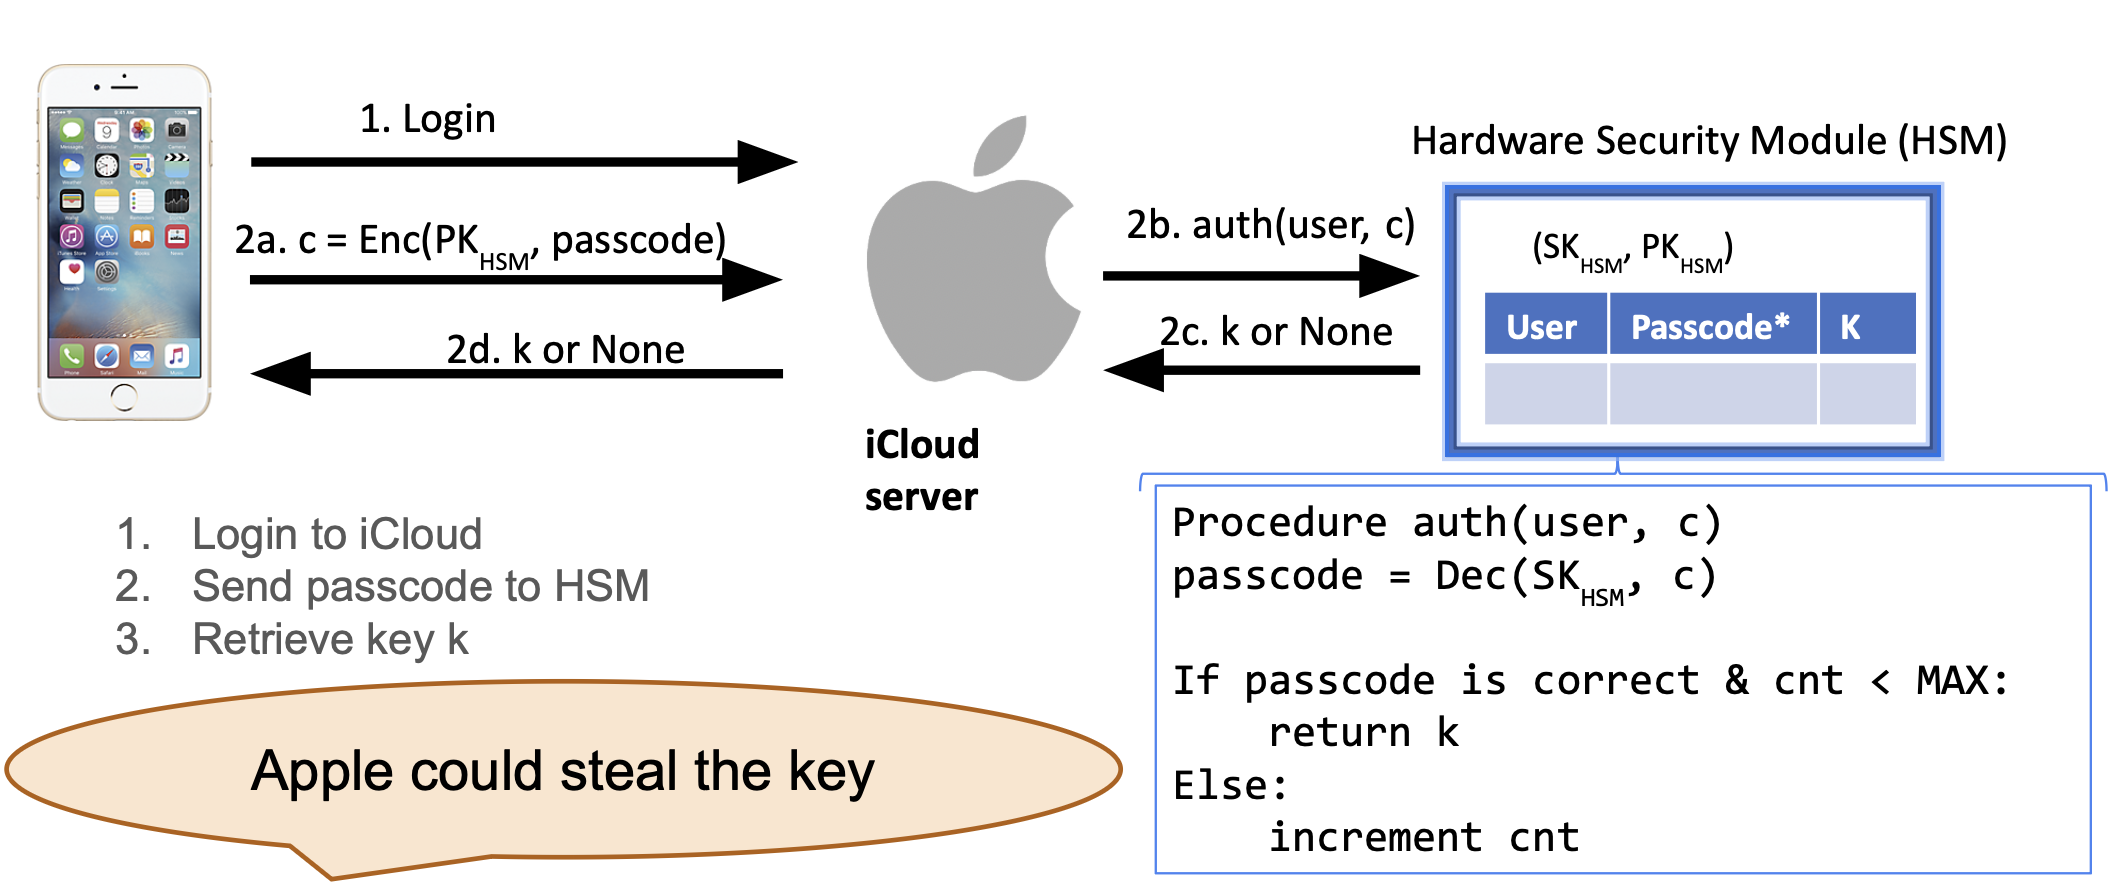
\includegraphics[width=0.8\textwidth]{apple-solution}
    \label{fig:LABEL}
\end{figure}

\subsection*{Apple's Secure Backup Solution: Retrieving Key}

% Quick centered image
\begin{figure}[H]
    \centering
    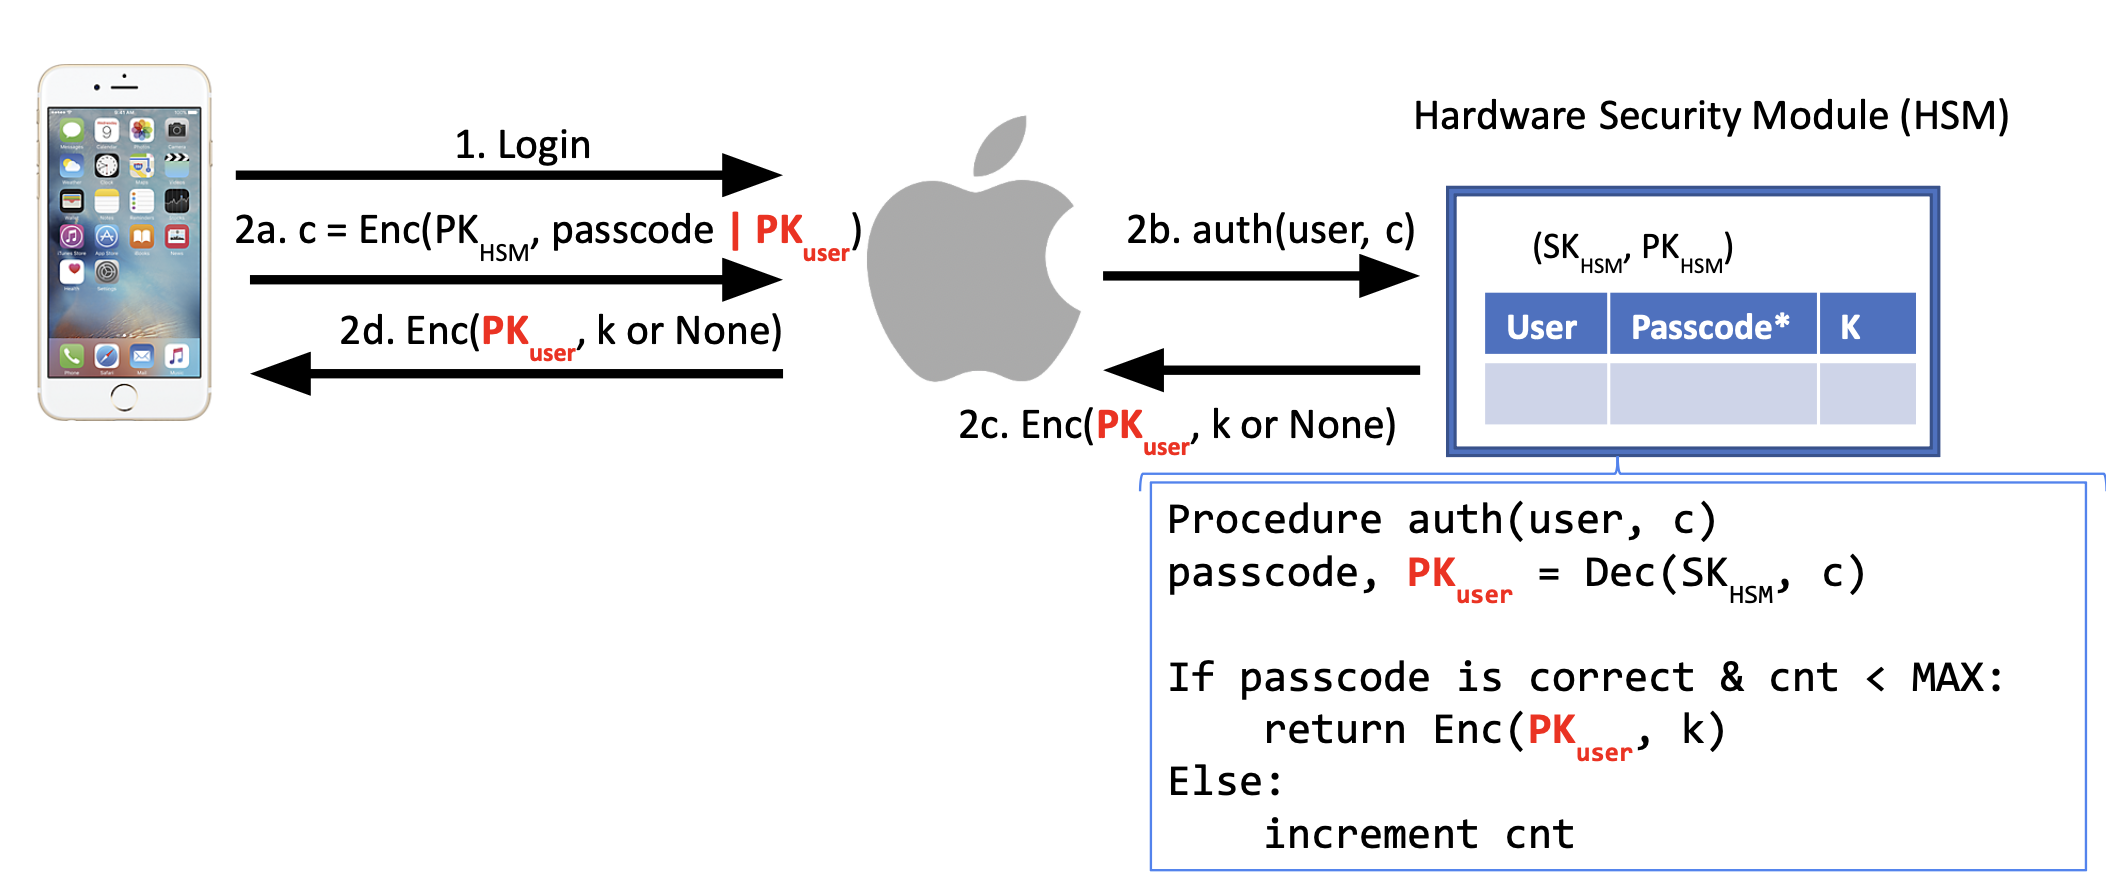
\includegraphics[width=0.8\textwidth]{apple-backup-sol}
    \label{fig:LABEL}
\end{figure}

\subsection*{Apple's Secure Backup: Protecting Software}

Apple's HSMs run custom software. This software can be update 

\begin{center}
	\textit{How to protect this software?}
\end{center}

1. Protect access keys: Apple's HSMs require smartcards to update, stored in sealed and tamper-evident bags while not used

2. Install software

3. Physically destroy access cards

\begin{tcolorbox}[
  colback=orange!15,     % background color
  colframe=black!50,    % border color
  boxrule=1pt,       % border thickness
  arc=3mm,             % rounded corners
  left=4mm, right=4mm, top=2mm, bottom=2mm % padding
]
Still need to trust Apple to install secure software in the first place
\end{tcolorbox}
\section*{Smartcards}

Plastic card with embedded integrated circuits which can process data and are often tamper resistant. Two main types:

\begin{itemize}
	\item Memory cards
	\item Microprocessor cards
\end{itemize}

Contain keys and certificates: Authentication / digital signatures, confidentiality, key management protocols

\subsection*{Use-case: Offline Payments}

Problem statement: we want users to be able to signal to the bank to pay to a merchant without talking to the bank. 

\begin{minipage}{0.4\textwidth}
Threat Model:  \\
\begin{itemize}
	\item Other users \\
	\item Merchant \\
	\item User herself \\
	\item External parties \\
\end{itemize}

Adversaries may have a lot of computational power and time!!
\end{minipage}
\hfill
\begin{minipage}{0.5\textwidth}
\centering
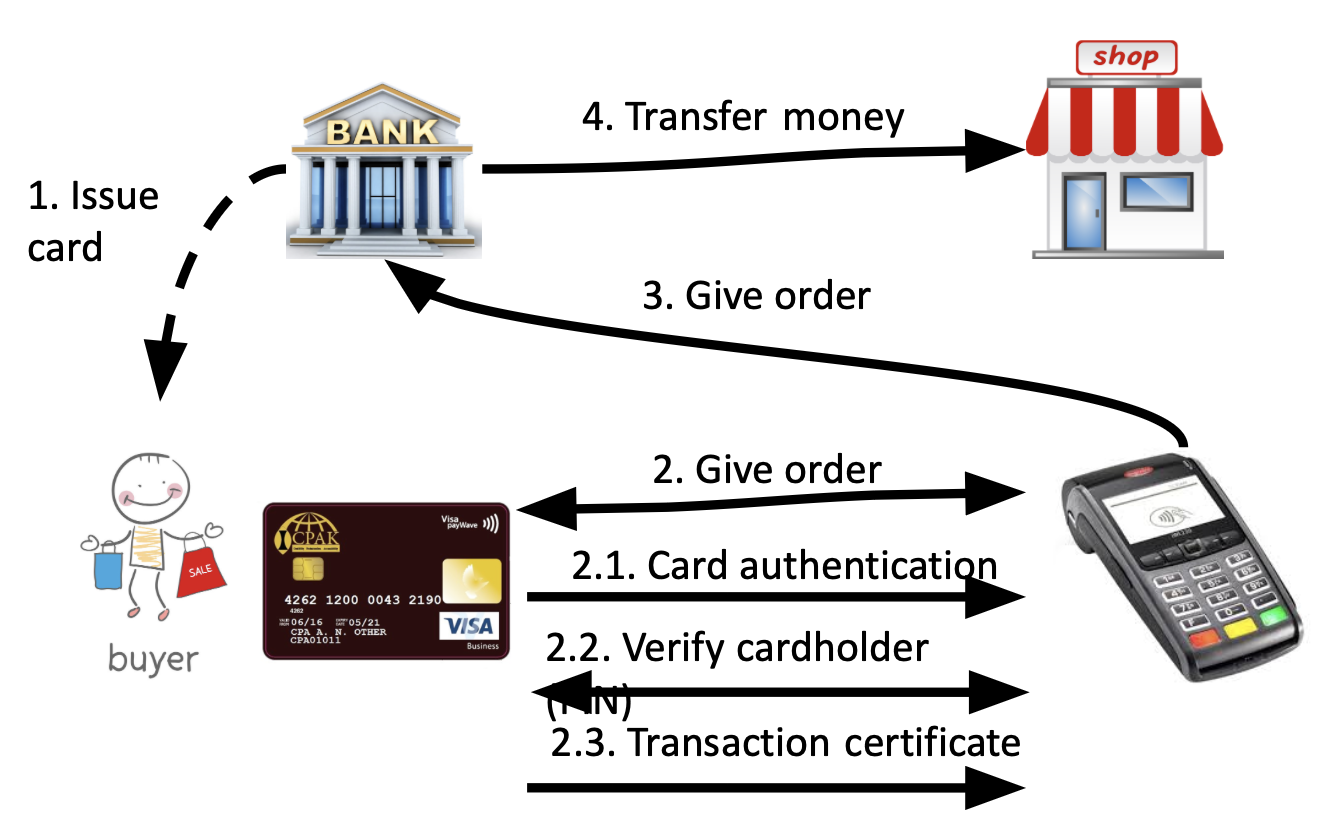
\includegraphics[width=\linewidth]{bank}
\end{minipage}
\vspace{0.5cm}

\subsection*{Static Data Authentication}

\begin{minipage}{0.4\textwidth}
\textbf{Solution 1: Static Data Authentication} \\
Problem: \textbf{\textit{Information can be copied}} \\
No freshness $\Rightarrow$ Replay is possible! \\
PIN verification unauthenticated, accept any PIN (YesCard) \\
Problem: \textbf{\textit{Signature can be forged!}}
\end{minipage}
\hfill
\begin{minipage}{0.5\textwidth}
\centering
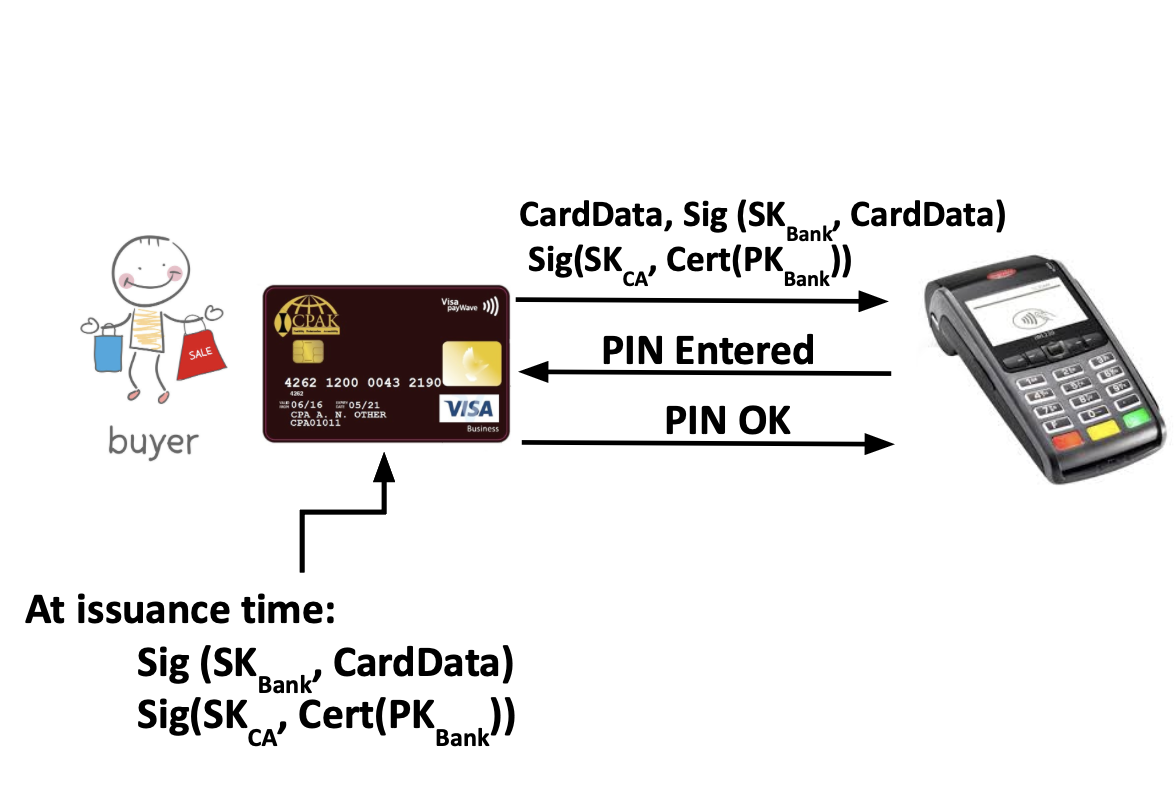
\includegraphics[width=\linewidth]{bank2}
\end{minipage}
\subsection*{Dynamic Data Authentication}
\begin{minipage}{0.4\textwidth}
\textbf{Solution 2: Dynamic Data Authentication} \\
Problem: \textbf{\textit{PIN verification unauthenticated}}: just accept any PIN (YesCard) \\
\textcolor{green}{Solution} Online checking solves these problems because data will not match, but it is an expensive process, with a risk of money loss
\end{minipage}
\hfill
\begin{minipage}{0.5\textwidth}
\centering
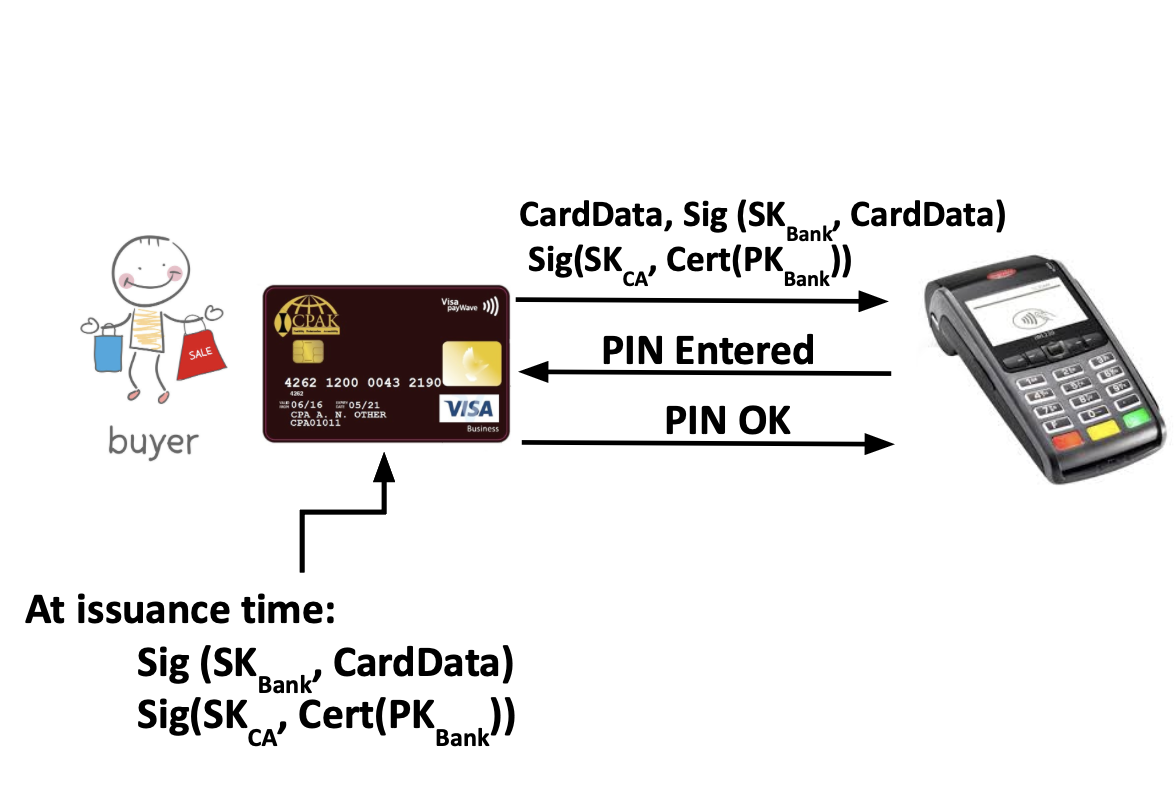
\includegraphics[width=\linewidth]{bank2}
\end{minipage}

\newpage
\begin{center}
  {\LARGE \textbf{Side channels}} \\
  Nightmare for trusted hardware
\end{center}
\vspace{0.5cm}

Running a program is a \textbf{real} thing
\begin{itemize}
	\item It takes \textbf{time}
	\item It takes \textbf{power}
	\item \textbf{Electromagnetic Emission}
\end{itemize}

\begin{tcolorbox}[
  colback=yellow!15,     % background color
  colframe=black!50,    % border color
  boxrule=1pt,       % border thickness
  arc=3mm,             % rounded corners
  left=4mm, right=4mm, top=2mm, bottom=2mm % padding
]
Can we exploit \underline{\textbf{unintentional leakages}} from hardware or software to learn secrets?
\end{tcolorbox}

\subsection*{Timing Attacks}

RSA decryption: compute $c^{d}$ mod N. A \textcolor{red}{modular exponentiation} operation

\textbf{Naive algorithm:} \textcolor{red}{square and multiply}

% Quick centered image
\begin{figure}[H]
    \centering
    \includegraphics[width=0.8\textwidth]{rsa}
    \label{fig:LABEL}
\end{figure}

Whether iteration takes a long time depends on the k$\_$th bit of secret exponent.

Computing $(c \cdot s)$ $mod$ $n$ \textcolor{red}{takes a while} but $R_k = s_k$ \textcolor{red}{is instantaneous}

\begin{tcolorbox}[
  colback=yellow!15,     % background color
  colframe=black!50,    % border color
  boxrule=1pt,       % border thickness
  arc=3mm,             % rounded corners
  left=4mm, right=4mm, top=2mm, bottom=2mm % padding
]
Timing depends on number of 1's 
\end{tcolorbox}

\subsection*{Power Analysis}

Elliptic-curve cryptography operation. Power depends on key bits. This could be analysed with a Oscilloscope. 

\subsection*{Electromagnetic Emissions}

Key Extraction from Mobile Devices via Non intrusive Physical Side Channels

\subsection*{Countermeasures Against Side Channels}

Goal: Prevent secret inference from observable state

\textbf{Hiding}: lowers signal to noise ration 

Noise generator, randomized execution order, asynchronous logic styles. ...

\textbf{Masking}: (secret sharing) splits state into shares; forces adversary to recombine

Boolean or arithmetic masking, Higher-order masking

\textbf{Leakage Resilience}: prevents leakage aggregation by updating secret


\section*{Micro-architectural Side Channels}

\subsection*{Meltdown}

Catastrophic attack making it possible to \textcolor{red}{read all memory of a process} (including \textcolor{red}{\textbf{protected kernel data}})

By-product of the way some micro-architectural features are implemented (e.g., AMD x86 implementations are \textbf{\textcolor{red}{per chance}} resistant to Meltdown)

Exploits \textcolor{red}{\textbf{race condition}} between \textcolor{red}{\textbf{memory access}} and \textbf{\textcolor{red}{protection checks}}

Ultimately exploits the micro-architectural nature of caches (something is left in the cache upon exception because \textcolor{red}{\textbf{the cache is not part of the architectural state}}

\begin{tcolorbox}[
  colback=yellow!15,     % background color
  colframe=black!50,    % border color
  boxrule=1pt,       % border thickness
  arc=3mm,             % rounded corners
  left=4mm, right=4mm, top=2mm, bottom=2mm % padding
]
The attacker executes a \textcolor{red}{\textbf{forbidden access}} and \textbf{\textcolor{red}{speculatively uses the result}} to obtain \textbf{\textcolor{red}{non-architectural side-effects}} that reveal the secrets \textbf{\textcolor{red}{before the forbidden access is squashed}}.
\end{tcolorbox}

\subsection*{Mapping Kernel Pages in User Space}

Most OSes mapped physical kernel memory pages into every user's virtual memory space

% Quick centered image
\begin{figure}[H]
    \centering
    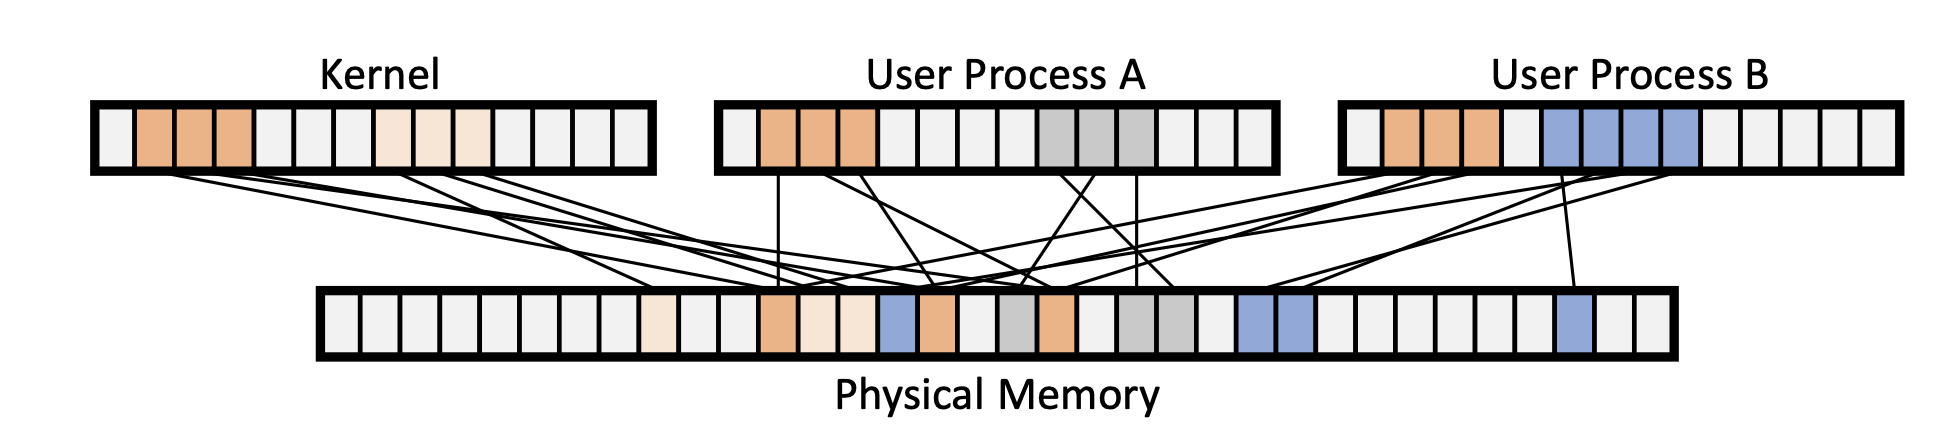
\includegraphics[width=0.8\textwidth]{kernel}
    \label{fig:LABEL}
\end{figure}

Minimizes the cost of some exceptions (e.g., fast interrupt handling, less TLB flushes)

Of course, \textcolor{red}{access is protected}, i.e., data can be read only in kernel mode

But \textcolor{red}{everyone can address them}!

% Quick centered image
\begin{figure}[H]
    \centering
    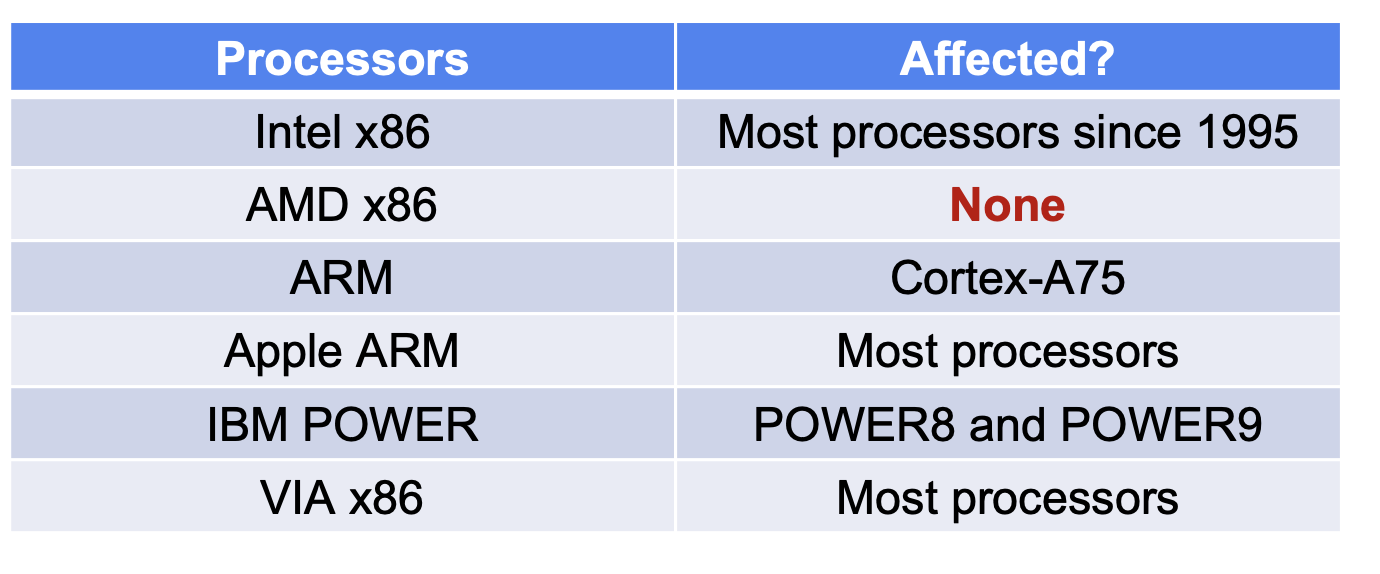
\includegraphics[width=0.8\textwidth]{processors}
    \label{fig:LABEL}
\end{figure}

\subsection*{Possible Mitigations}

The obvious proper solutions it to \textbf{\textcolor{red}{change the processor design}}
\begin{itemize}
	\item Test privilege level \textbf{\textcolor{red}{before}} making the result of a speculative access available
	\item By chance, AMD does this already
\end{itemize}

The other line of mitigation is to \textbf{\textcolor{red}{isolate user space and kernel}} space memory
\begin{itemize}
	\item In Linux, \textbf{\textcolor{red}{Kernel page-table isolation (KPTI)}}: similar in other OSes
	\item Performance penalty in Linux around 5-10\%, up to 30\%
\end{itemize}

\subsection*{Spectre}

Another catastrophic attack making it possible to \textbf{\textcolor{red}{read all memory}}.

Addresses another shared resource: \textbf{\textcolor{red}{branch predictors}}

\begin{itemize}
	\item For simplicity, brand predictors are not unique per-thread (but shared among SMT threads)
\end{itemize}

Exploits side effects of \textbf{\textcolor{red}{(miss-predicted) speculative execution}}
\begin{itemize}
	\item Mispeculation does not affect the architectural state (of course!)...
	\item ...but it may \textcolor{red}{\textbf{affect micro-architectural structures}} (e.g., caches)
\end{itemize}

\begin{tcolorbox}[
  colback=yellow!15,     % background color
  colframe=black!50,    % border color
  boxrule=1pt,       % border thickness
  arc=3mm,             % rounded corners
  left=4mm, right=4mm, top=2mm, bottom=2mm % padding
]
Get the victim to \textbf{\textcolor{red}{speculatively}} execute \textbf{\textcolor{red}{leaky}} code whose \textbf{\textcolor{red}{non-architectural side-effects}} reveal the secrets
\end{tcolorbox}

\subsection*{Possible Mitigations}

\textbf{Hardware}
\begin{itemize}
	\item Disable speculative execution
	\item Separate branch predictors per process/thread
\end{itemize}

\textbf{General software} approaches
\begin{itemize}
	\item Run only an application per processor
\end{itemize}

\textbf{Partial and application-specific software} approaches
\begin{itemize}
	\item Add serialization instructions between branches and loads
	\item Make it impossible through JavaScript in browsers
\end{itemize}

\textbf{Not easy to fix!}


\section*{Even With Trusted Hardware, Vendor Requires \textbf{\textit{Some}}} Trust

\textbf{Backup data system from Apple}

\textbf{HSM manufacturer}: controls the production of the "black box"

\textbf{Apple}: Must be trusted to install the correct code the first time (attestation helps)

\textbf{Discovery of private contacts for Signal (based on Intel SGX)}

\textbf{Intel}: Controls the production of the (black box) SGX system. It also controls the attestation keys built into every device.

\textbf{Signal}: Must be trusted to not leak any data from the mobile application but not for running the correct set intersection code (the attestation allows to check that)


\section*{Trusted Hardware: Lessons Learned}

It exits, and offers three properties:
\begin{itemize}
	\item \textbf{Isolation}: it is not possible to "peek" inside
	\item \textbf{Attestation}: it can prove that it does what you think it is doing
	\item \textbf{Sealing}: it can store secrets in memory that can only be recovered by itself
\end{itemize}

\begin{tcolorbox}[
  colback=orange!15,     % background color
  colframe=black!50,    % border color
  boxrule=1pt,       % border thickness
  arc=3mm,             % rounded corners
  left=4mm, right=4mm, top=2mm, bottom=2mm % padding
]
Having trusted hardware doesn't mean you don't need to think about protocols!
\end{tcolorbox}

Building trusted hardware is difficult: side channel attacks

Trusted hardware means to trust the manufacturer!

Separation of privilege: Use several cards with advanced cryptography.
\end{document}
